\documentclass[12pt]{ctexart}
\usepackage{geometry}
\geometry{a4paper, margin=1in}
\usepackage{amsmath}
\usepackage{graphicx}
\usepackage{multirow}
\usepackage{setspace}
\usepackage{caption}
\usepackage{float}
\usepackage{booktabs}
\usepackage{verbatim}
\usepackage{hyperref}
\usepackage{xcolor}
\usepackage{listings}
\usepackage{tabularx}
\usepackage{longtable}
% 格式设置
\renewcommand{\arraystretch}{1.5} % 行高调整为1.5倍
\setlength{\tabcolsep}{4pt} % 列间距调整为4pt

\setstretch{1.5}          % 1.5倍行距
\setlength{\parindent}{2em} % 首行缩进2字符

% 封面模板
\newcommand{\cover}[6]{
  \begin{center}
    {\LARGE \bfseries 《分布式能源系统概论》}\\[1em]
    {\Large 实践作业}\\[2em]
    
    \begin{tabular}{ll}
      作业题目: & \underline{\makebox[8cm][s]{#1}} \\
      专~~~~业: & 能源与动力工程 \\
      班~~~~级: & 2023级能源与动力工程一班(化能杨班) \\
      学生姓名: & 唐玮嘉 \\
      学~~~~号: & 2023428020130 \\
      指导教师: & 陶实 副教授 \\
      年~月~日: & \underline{\makebox[4cm][s]{#2}} \\
    \end{tabular}
  \end{center}
  \vspace{2em}
}

\begin{document}

% 封面
\cover{基于EPTE指标的冷热电联供系统经济性比较分析}{\today}

% 课程论文任务书
\section*{课程论文任务书}
专业:能源与动力工程 \quad 班级:2023级能源与动力工程一班(化能杨班)


\begin{tabularx}{\textwidth}{|l|X|X|X|} % 使用全页面宽度
  \hline
  学生姓名 & 唐玮嘉 & 学号 & 2023428020130 \\
  \hline
  论文题目 & \multicolumn{3}{X|}{\underline{基于EPTE指标的冷热电联供系统经济性比较分析}} \\
  \hline
  % --- ADJUSTED THIS LINE ---
  \multirow{3}{*}{\begin{tabular}[c]{@{}l@{}}设计目的、\\主要内容\\及要求\end{tabular}}
    % --- END OF ADJUSTMENT ---
    & 论文目的: & \multicolumn{2}{X|}{\begin{minipage}[t]{\hsize}
        研究冷热电联供系统的经济性,通过EPTE指标对两种燃气轮机和燃气内燃机进行经济性比较分析,探讨其各自的经济适用范围。
    \end{minipage}} \\
    \cline{2-4} % 横跨三列
    & 主要内容: & \multicolumn{2}{X|}{\begin{minipage}[t]{\hsize}
      1. 引言:简述分布式能源及冷热电联供的背景意义,引出经济性评价及EPTE指标。
      2. EPTE计算模型:详细介绍EPTE的定义、计算公式,包括发电收益、供热收益、燃料成本、维修成本的计算方法,以及热价的确定方法。
      3. 基础数据与参数拟合:说明燃气轮机和燃气内燃机的主要性能参数数据来源。
    \end{minipage}} \\
    \cline{2-4} % 横跨三列
    & 要求: & \multicolumn{2}{X|}{\begin{minipage}[t]{\hsize}
      1. 统一使用A4纸打印;\\
      2. 论文撰写格式请参考附录。(实际按本模板格式撰写) \\
      3. 数据处理和图表绘制要求清晰、规范,分析合理。
    \end{minipage}} \\
  \hline
  进度安排 & \multicolumn{3}{|l|}{\begin{tabular}{l}
    % 根据要求,此处留空
  \end{tabular}} \\
  \hline
  主要参考资料 & \multicolumn{3}{|l|}{\begin{minipage}[t]{0.9\textwidth}
    \begin{enumerate}
      \item 《分布式冷热电联产系统装置及应用》,金红光等主编,中国电力出版社,2010年
      \item 《小型吸收式制冷机原理与应用》,王林主编,中国建筑工业出版社,2011年
      \item 《燃气冷热电分布式能源技术应用手册》,林世平等主编,中国电力出版社,2014年
    \end{enumerate}
  \end{minipage}} \\
  \hline
  指导教师签字 & \multicolumn{3}{|l|}{\underline{\makebox[12cm][s]{}}} \\
  \hline
\end{tabularx}


% 摘要与关键词
\section*{摘 要}
\noindent 本文旨在通过热电性能经济参数(EPTE)对燃气轮机和燃气内燃机两种冷热电联供系统的经济性进行比较研究。首先,详细阐述了EPTE的计算模型,包括发电收益、供热收益、燃料成本、维修成本以及热价的确定方法。其次,基于课程提供的机组性能数据,利用Origin软件对燃气轮机和燃气内燃机的发电效率、热电效率、单位维修费用和机组价格随额定功率的变化规律进行多项式拟合,得到了相应的经验公式。在此基础上,设定了年运行5000小时的工况,并考虑了两种对比分析情景:(1) 电价分别为0.6元/kWh和0.8元/kWh(天然气价格固定为2.5元/m³);(2) 天然气价格分别为2.5元/m³和3.5元/m³(电价固定为0.6元/kWh)。通过计算和绘制EPTE随额定功率变化的曲线,对比分析了不同能源价格和功率等级下两种机组的经济适用性。研究结果将揭示不同类型机组在特定条件下的经济优势区间,为分布式能源系统的选型和优化提供参考。

\section*{关键词}
\noindent 冷热电联供;EPTE;经济性分析;燃气轮机;燃气内燃机;Origin拟合;能源价格

\newpage
% 目录
\tableofcontents
\addcontentsline{toc}{section}{目 录} % 添加目录到目录页

\newpage
% 正文
\section{引言}
随着能源结构的转型和环境保护要求的日益提高,分布式能源系统因其能源利用效率高、环境友好、供能可靠性强等优点,受到了广泛关注与应用。冷热电联供(CCHP)作为一种重要的分布式能源系统形式,能够根据用户需求同时提供电、热、冷三种能源,实现了能源的梯级利用,具有显著的节能和减排效益。

在CCHP系统的规划与设计中,经济性是决定项目可行性的关键因素之一。热电性能经济参数 (EPTE) 是一种综合评价CCHP系统经济性的指标,它综合考虑了系统的初投资、运行成本(燃料、维修)以及能源产出(电、热)的收益。通过EPTE分析,可以对不同类型、不同容量的CCHP机组在特定能源价格和运行策略下的经济表现进行量化比较,为系统选型提供科学依据。

本次作业旨在采用EPTE指标,对市场上常见的燃气轮机和燃气内燃机两种CCHP原动机进行经济性对比分析。将利用Origin软件对机组的关键性能参数进行曲线拟合,并在不同的电价和天然气价格情景下,计算和比较两种机组的EPTE值,探讨其各自的经济适用范围。

\section{EPTE计算模型}
\subsection{2.1 EPTE定义}
热电性能经济参数EPTE定义为系统的年净收益与机组初投资的比值,反映了单位投资的盈利能力或投资回收的快慢程度。其基本计算公式如下:
\[
\text{EPTE} = \frac{\text{年净收益}}{\text{机组价格}} = \frac{\text{年总收益} - \text{年总支出}}{\text{机组价格}}
\]
其中:
\begin{itemize}
    \item 年总收益 = 年发电收益 + 年供热收益
    \item 年总支出 = 年燃料支出 + 年维修支出
\end{itemize}

\subsection{2.2 各分项计算}
假设机组年运行小时数为 $T$ (h/year)。
\begin{enumerate}
    \item \textbf{年发电量 ($E_{gen}$)}:
    \[ E_{gen} = P_{rated} \times T \quad (\text{kWh/year}) \]
    其中 $P_{rated}$ 为机组额定发电功率 (kW)。

    \item \textbf{年发电收益 ($R_{elec}$)}:
    \[ R_{elec} = E_{gen} \times C_{elec} \quad (\text{元/year}) \]
    其中 $C_{elec}$ 为上网电价或用户侧替代电价 (元/kWh)。

    \item \textbf{年供热量 ($Q_{supply}$)}:
    机组的供热功率 $P_{heat}$ 可由发电功率 $P_{rated}$、发电效率 $\eta_e$ 和热电效率 $\eta_{th}$ 计算得到:
    \[ P_{heat} = P_{rated} \times \frac{\eta_{th} - \eta_e}{\eta_e} \quad (\text{kW}) \]
    则年供热量为:
    \[ Q_{supply} = P_{heat} \times T = E_{gen} \times \frac{\eta_{th} - \eta_e}{\eta_e} \quad (\text{kWh/year}) \]
    这里 $\eta_e$ 和 $\eta_{th}$ 均为随 $P_{rated}$ 变化的函数。

    \item \textbf{热价 ($C_{heat}$)}:
    热价通常参考等效的燃气锅炉产热成本确定:
    \[ C_{heat} = \frac{C_{fuel}}{\text{HV}_{ng, kWh} \times \eta_{boiler}} \quad (\text{元/kWh}) \]
    其中:
    \begin{itemize}
        \item $C_{fuel}$ 为天然气价格 (元/m³)。
        \item $\text{HV}_{ng, kWh}$ 为天然气低位热值,单位转换为 kWh/m³ (例如,35200 kJ/m³ $\approx$ 9.778 kWh/m³)。
        \item $\eta_{boiler}$ 为燃气锅炉效率 (例如,取0.85)。
    \end{itemize}

    \item \textbf{年供热收益 ($R_{heat}$)}:
    \[ R_{heat} = Q_{supply} \times C_{heat} \quad (\text{元/year}) \]

    \item \textbf{年燃料消耗量 ($V_{fuel}$)}:
    \[ V_{fuel} = \frac{E_{gen}}{\eta_e \times \text{HV}_{ng, kWh}} \quad (\text{m³/year}) \]

    \item \textbf{年燃料支出 ($C_{f,total}$)}:
    \[ C_{f,total} = V_{fuel} \times C_{fuel} \quad (\text{元/year}) \]

    \item \textbf{年维修支出 ($C_{m,total}$)}:
    \[ C_{m,total} = C_{maint\_rate} \times E_{gen} \quad (\text{元/year}) \]
    其中 $C_{maint\_rate}$ 为单位发电量的维修费用 (元/kWh),是随 $P_{rated}$ 变化的函数。

    \item \textbf{机组价格 ($IC$)}:
    机组价格通常指设备初投资 (元),是随 $P_{rated}$ 变化的函数。
\end{enumerate}

\section{基础数据与参数拟合}
\subsection{3.1 数据来源}
本研究中燃气轮机和燃气内燃机的性能参数(额定功率、发电效率、热电效率、维修费用率、机组价格)数据来源于课程提供的参考图表(参考类似教材中的表4-2和表4-3)。

\subsection{3.2 参数拟合方法}
为获得连续的性能参数随额定功率变化的函数关系,采用Origin软件对上述离散数据点进行多项式拟合。拟合目标参数包括:发电效率 $\eta_e(P)$,热电效率 $\eta_{th}(P)$,维修费用率 $C_{maint\_rate}(P)$,以及机组价格 $IC(P)$。根据提供的拟合结果信息,采用三阶多项式模型:
\[ y = A + B_1 \cdot P + B_2 \cdot P^2 + B_3 \cdot P^3 \]
其中 $y$ 为待拟合参数,$P$ 为额定发电功率 (kW),$A, B_1, B_2, B_3$ 为拟合系数。

\subsection{3.3 拟合系数}
根据提供的Origin拟合结果摘要 (基于OCR图片 `OCR\_多项式拟合1.png` 和 `OCR\_多项式拟合2.png`),燃气轮机 (GT) 和燃气内燃机 (ICE) 的主要性能参数拟合系数如下(请注意,效率值在计算时应转换为小数形式,价格单位可能需统一):

\textbf{燃气轮机 (GT) 拟合系数:}
\begin{itemize}
    \item 发电效率 $\eta_{e,GT}(P)$: $A=20.4623, B_1=-5.04871 \times 10^{-4}, B_2=6.41759 \times 10^{-8}, B_3=-1.13939 \times 10^{-12}$ (百分比)
    \item 热电效率 $\eta_{th,GT}(P)$: $A=66.64929, B_1=-5.90039 \times 10^{-4}, B_2=5.38413 \times 10^{-8}, B_3=-9.27892 \times 10^{-13}$ (百分比)
    \item 维修费用率 $C_{maint,GT}(P)$: $A=0.03006, B_1=6.92431 \times 10^{-8}, B_2=-2.55999 \times 10^{-12}, B_3=3.37218 \times 10^{-17}$ (元/kWh) (此处的维修费用拟合系数来自"维修费用"项,原数据单位可能需要确认是否为元/kWh)
    \item 机组价格 $IC_{GT}(P)$: $A=849.40872, B_1=1.71435, B_2=1.58074 \times 10^{-4}, B_3=-3.27059 \times 10^{-9}$ (千元)
\end{itemize}

\textbf{燃气内燃机 (ICE) 拟合系数:}
\begin{itemize}
    \item 发电效率 $\eta_{e,ICE}(P)$: $A=21.55525, B_1=0.0204, B_2=-9.11454 \times 10^{-6}, B_3=1.0748 \times 10^{-9}$ (百分比)
    \item 热电效率 $\eta_{th,ICE}(P)$: $A=80.92531, B_1=-0.02353, B_2=1.02267 \times 10^{-5}, B_3=-1.19163 \times 10^{-9}$ (百分比)
    \item 维修费用率 $C_{maint,ICE}(P)$: $A=0.33582, B_1=-4.503 \times 10^{-4}, B_2=1.72254 \times 10^{-7}, B_3=-1.8877 \times 10^{-11}$ (元/kWh) (此处的维修费用拟合系数来自"维修费用"项,原数据单位可能需要确认是否为元/kWh)
    \item 机组价格 $IC_{ICE}(P)$: $A=136.25293, B_1=0.14314, B_2=1.75 \times 10^{-3}, B_3=-2.66086 \times 10^{-7}$ (千元)
\end{itemize}
\textit{注意:上述系数中,效率的截距单位为\%,计算时需除以100。机组价格单位为千元,计算EPTE时需乘以1000。维修费用率的拟合数据来源和单位需仔细核对,确保其物理意义为 元/kWh。 }

\subsection{3.4 拟合曲线图示例}
为直观展示拟合效果,应给出关键参数(如发电效率、机组价格)的拟合曲线与原始数据点的对比图。
\begin{figure}[H]
  \centering
  % \includegraphics[width=0.8\textwidth]{placeholder.png} % 替换为实际图片
  %插入图片
  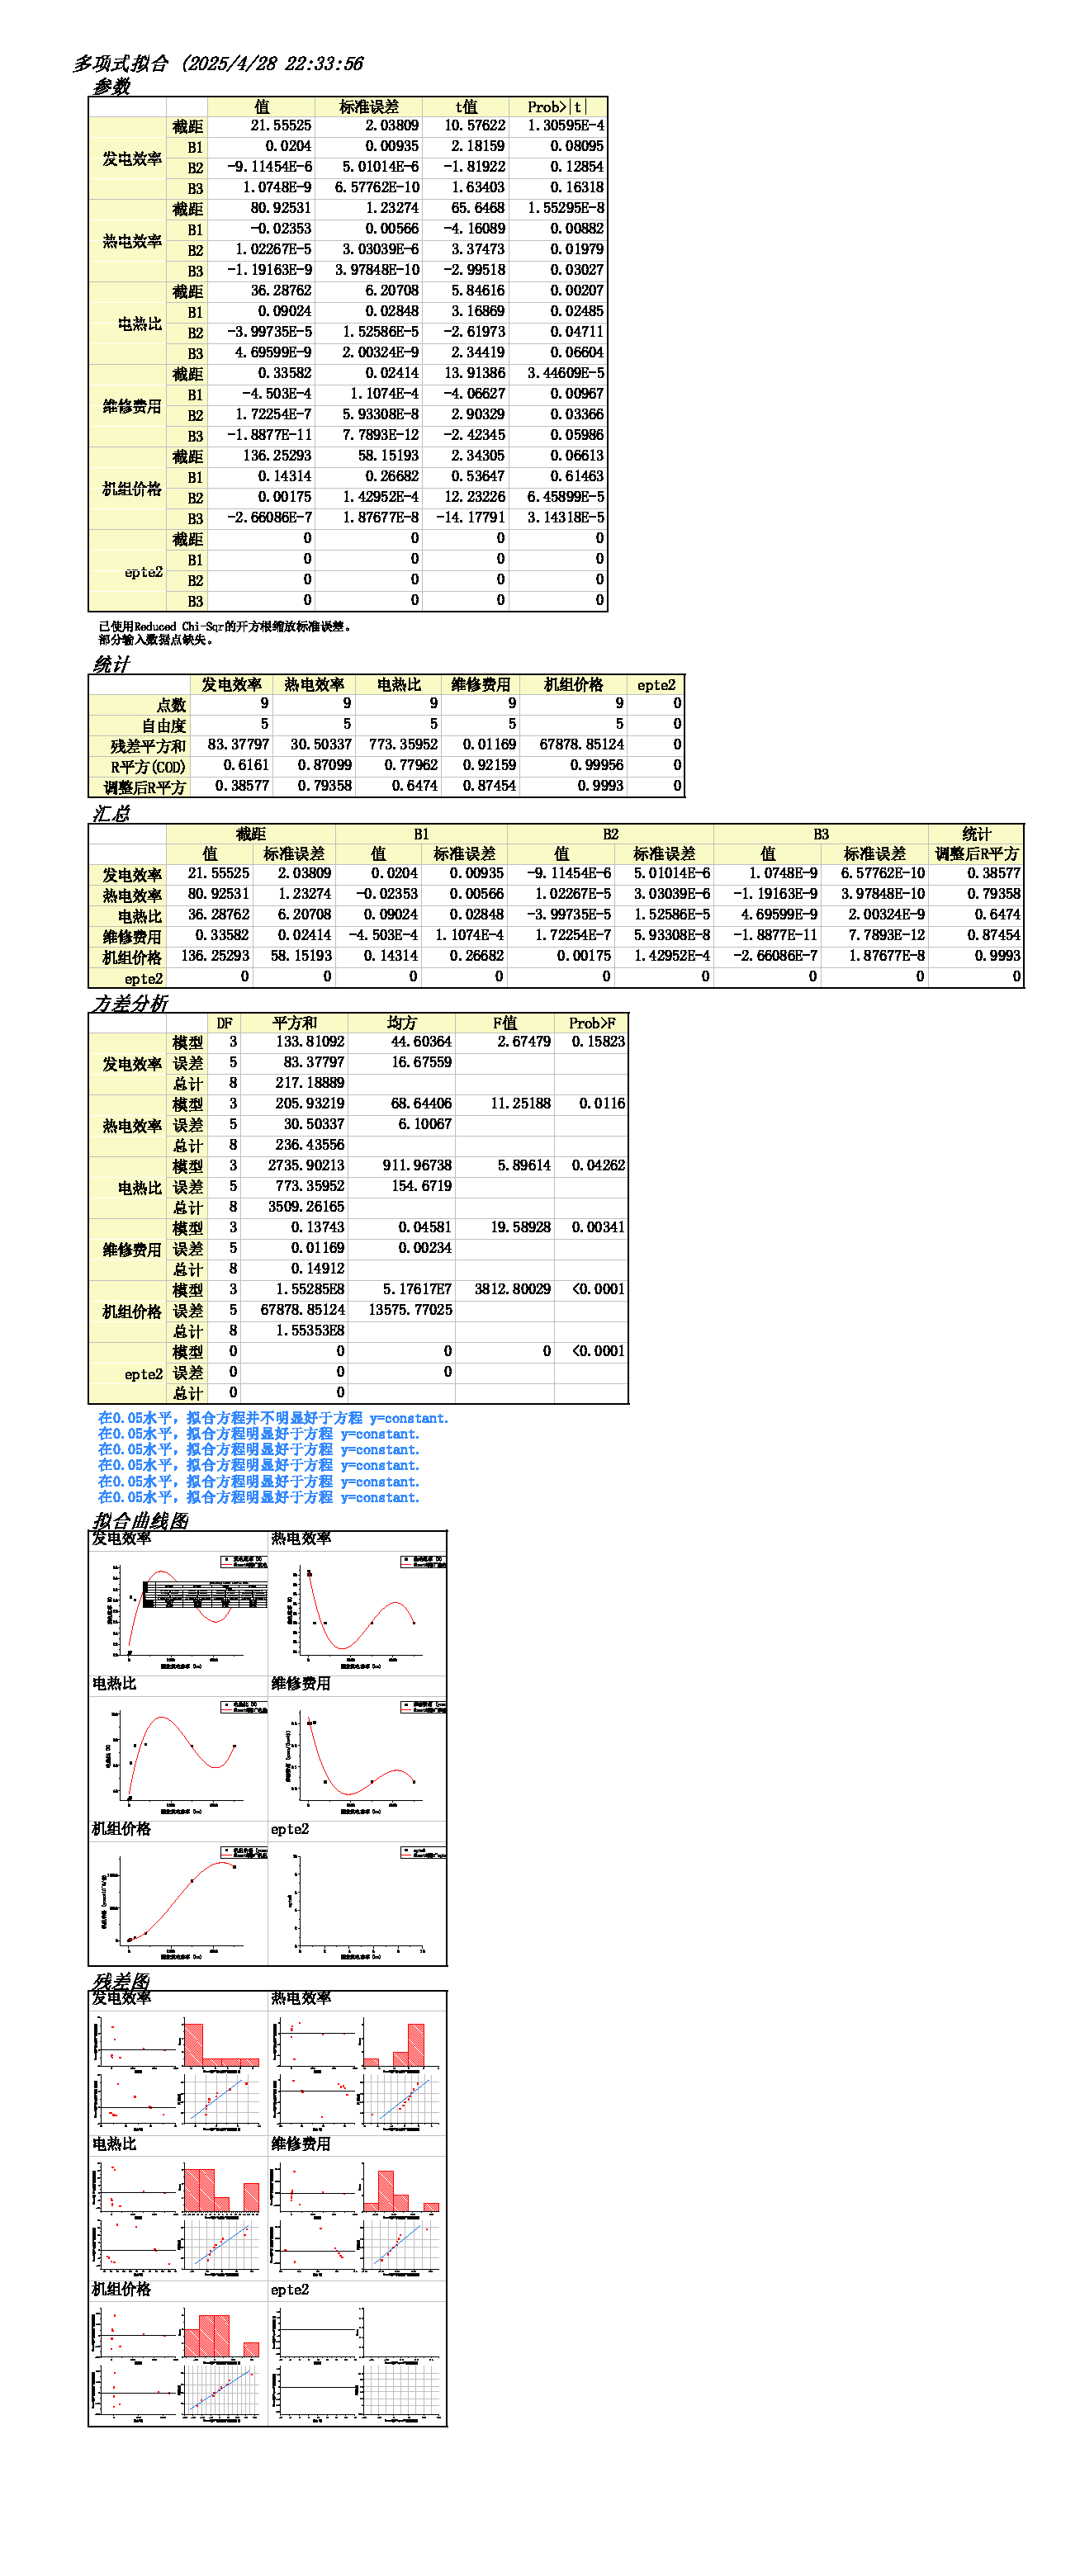
\includegraphics[width=0.8\textwidth]{fig/实践2_内燃机_拟合曲线.pdf} % 图片路径
  \caption{燃气轮机拟合曲线示例}
  \label{fig:price_fit}
\end{figure}

\begin{figure}[H]
  \centering
  % \includegraphics[width=0.8\textwidth]{placeholder.png} % 替换为实际图片
  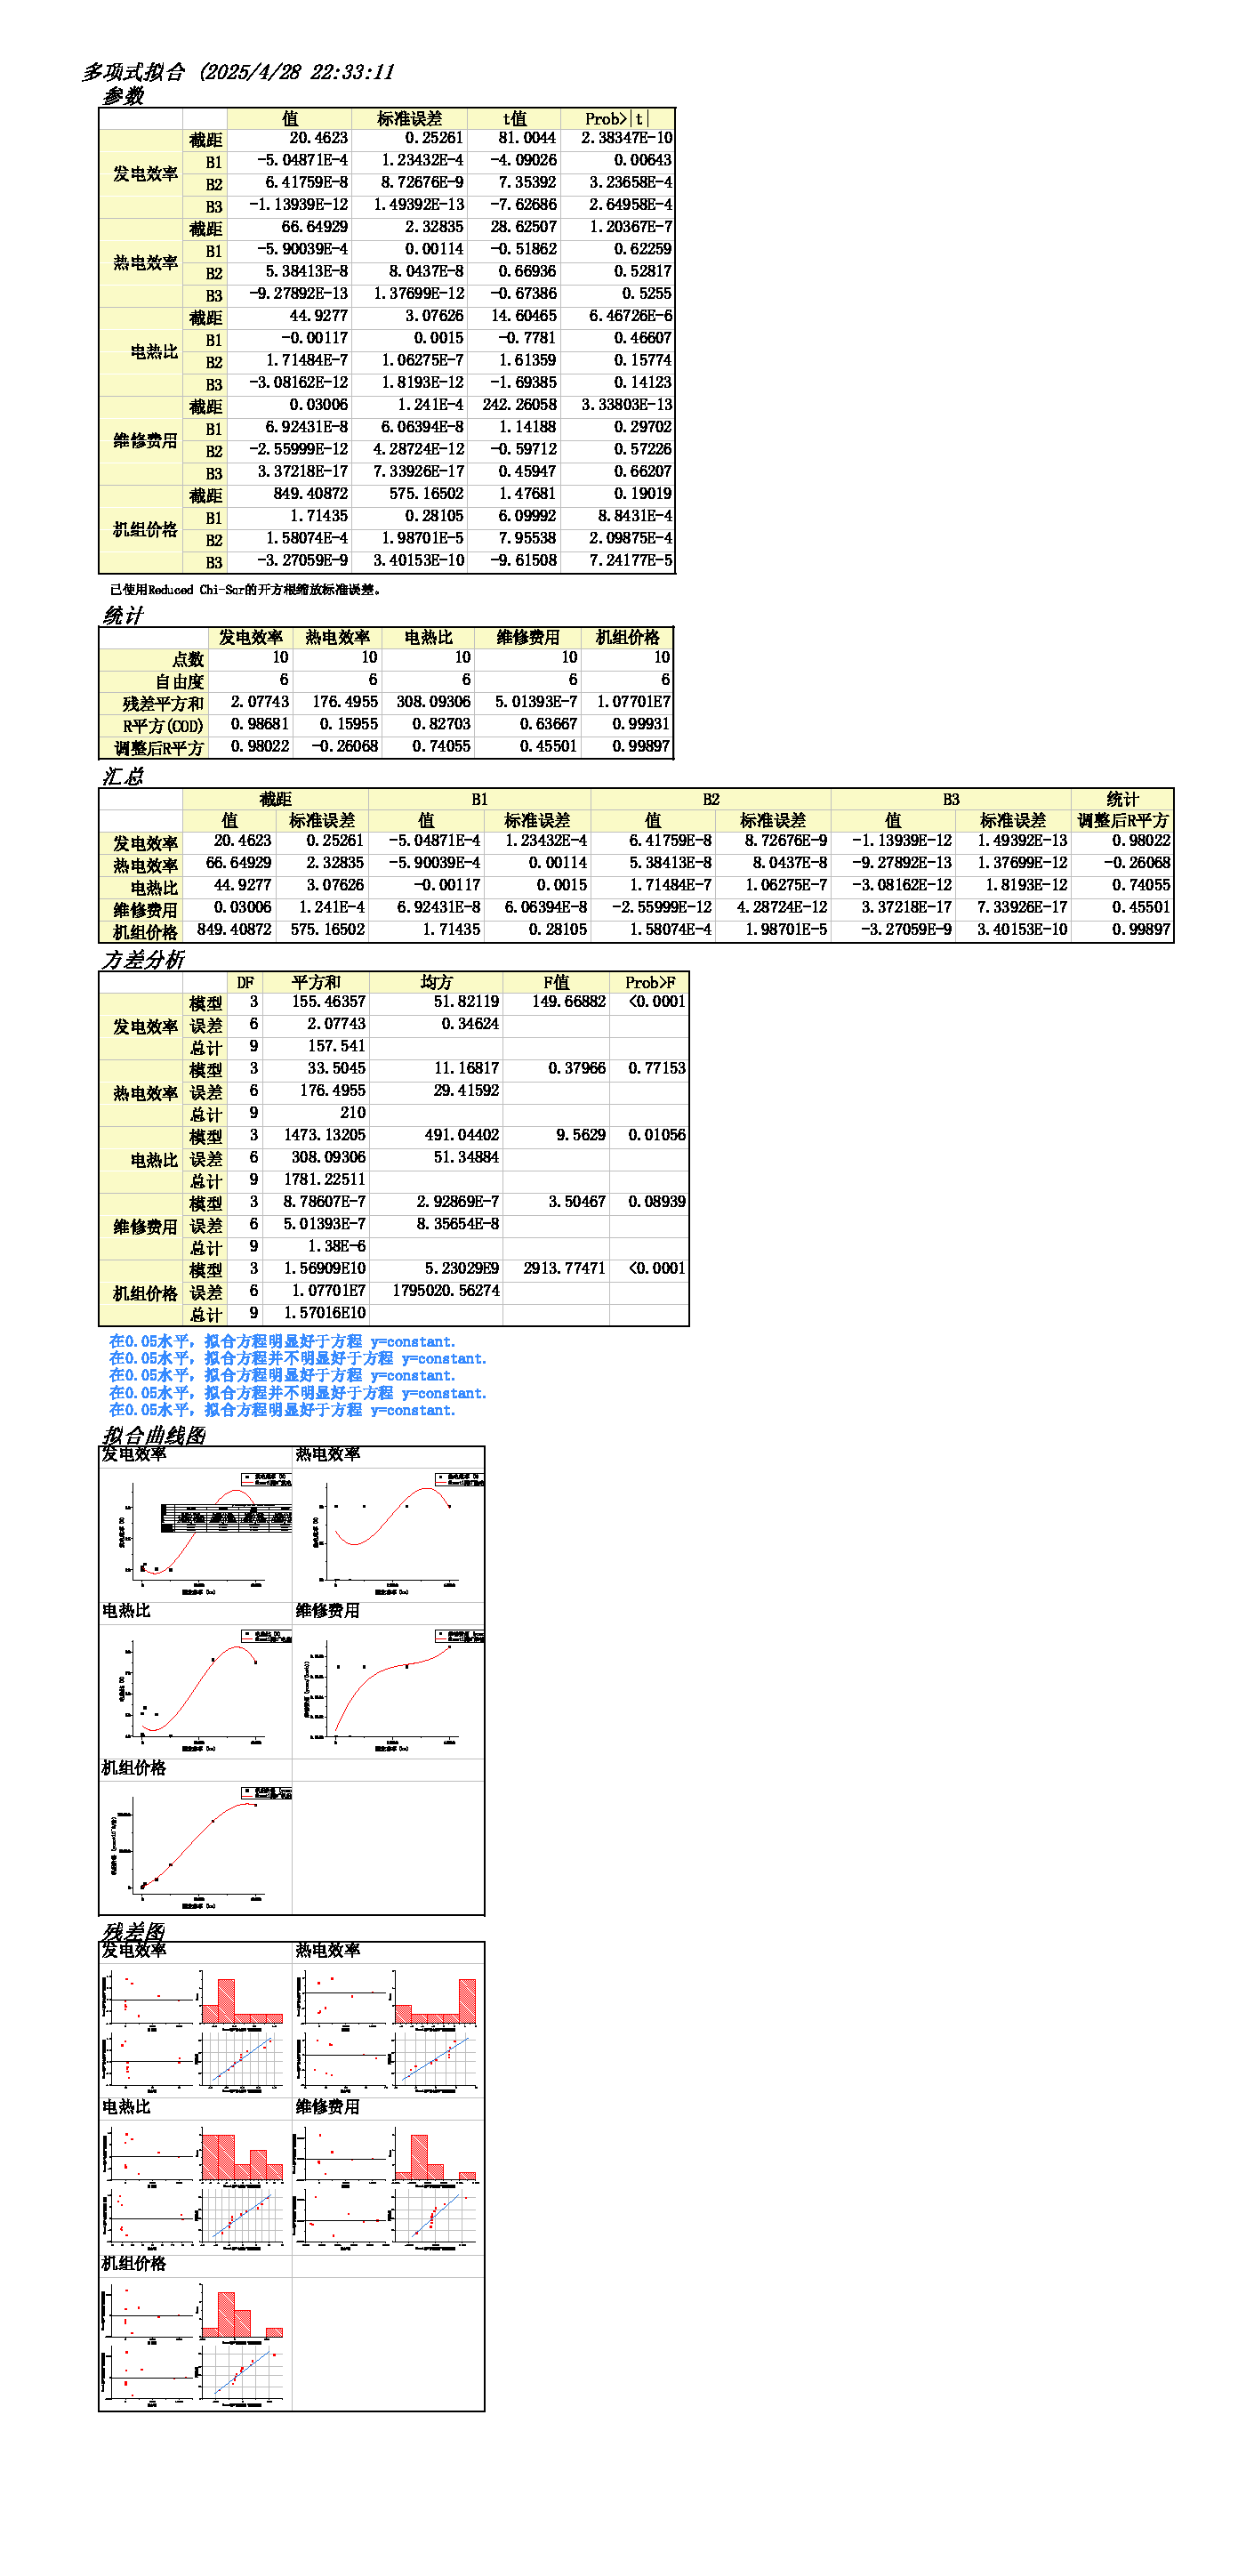
\includegraphics[width=0.8\textwidth]{fig/实践2_燃气轮机_拟合曲线.pdf} % 图片路径
  \caption{燃气轮机拟合曲线示例}
  \label{fig:price_fit}
\end{figure}


\section{案例分析与情景设置}
\subsection{4.1 计算参数}
\begin{itemize}
    \item 年运行小时数 $T = 5000$ h/year
    \item 天然气低位热值 $\text{HV}_{ng} = 35200$ kJ/m³ $\approx 9.778$ kWh/m³
    \item 燃气锅炉效率 $\eta_{boiler} = 0.85$
\end{itemize}

\subsection{4.2 分析情景}
为考察不同能源价格对两种机组经济性的影响,设定以下分析情景:
\begin{enumerate}
    \item \textbf{情景一:不同电价,天然气价格固定}
    \begin{itemize}
        \item 子情景1.1: 电价 $C_{elec} = 0.6$ 元/kWh, 天然气价格 $C_{fuel} = 2.5$ 元/m³
        \item 子情景1.2: 电价 $C_{elec} = 0.8$ 元/kWh, 天然气价格 $C_{fuel} = 2.5$ 元/m³
    \end{itemize}
    在此情景下,热价 $C_{heat,1} = 2.5 / (9.778 \times 0.85) \approx 0.300$ 元/kWh。

    \item \textbf{情景二:不同天然气价格,电价固定}
    \begin{itemize}
        \item 子情景2.1: 电价 $C_{elec} = 0.6$ 元/kWh, 天然气价格 $C_{fuel} = 2.5$ 元/m³ (同1.1)
        \item 子情景2.2: 电价 $C_{elec} = 0.6$ 元/kWh, 天然气价格 $C_{fuel} = 3.5$ 元/m³
    \end{itemize}
    在子情景2.2下,热价 $C_{heat,2} = 3.5 / (9.778 \times 0.85) \approx 0.421$ 元/kWh。
\end{enumerate}

\section{结果与讨论}
基于上述EPTE模型、拟合参数和情景设定,计算得到不同条件下燃气轮机和燃气内燃机的EPTE值随额定功率的变化情况。

\subsection{5.1 不同电价下的EPTE比较}
下图展示了在天然气价格为2.5元/m³时,电价分别为0.6元/kWh和0.8元/kWh的情况下,两种机组EPTE随功率的变化曲线。

\begin{figure}[H]
  \centering
  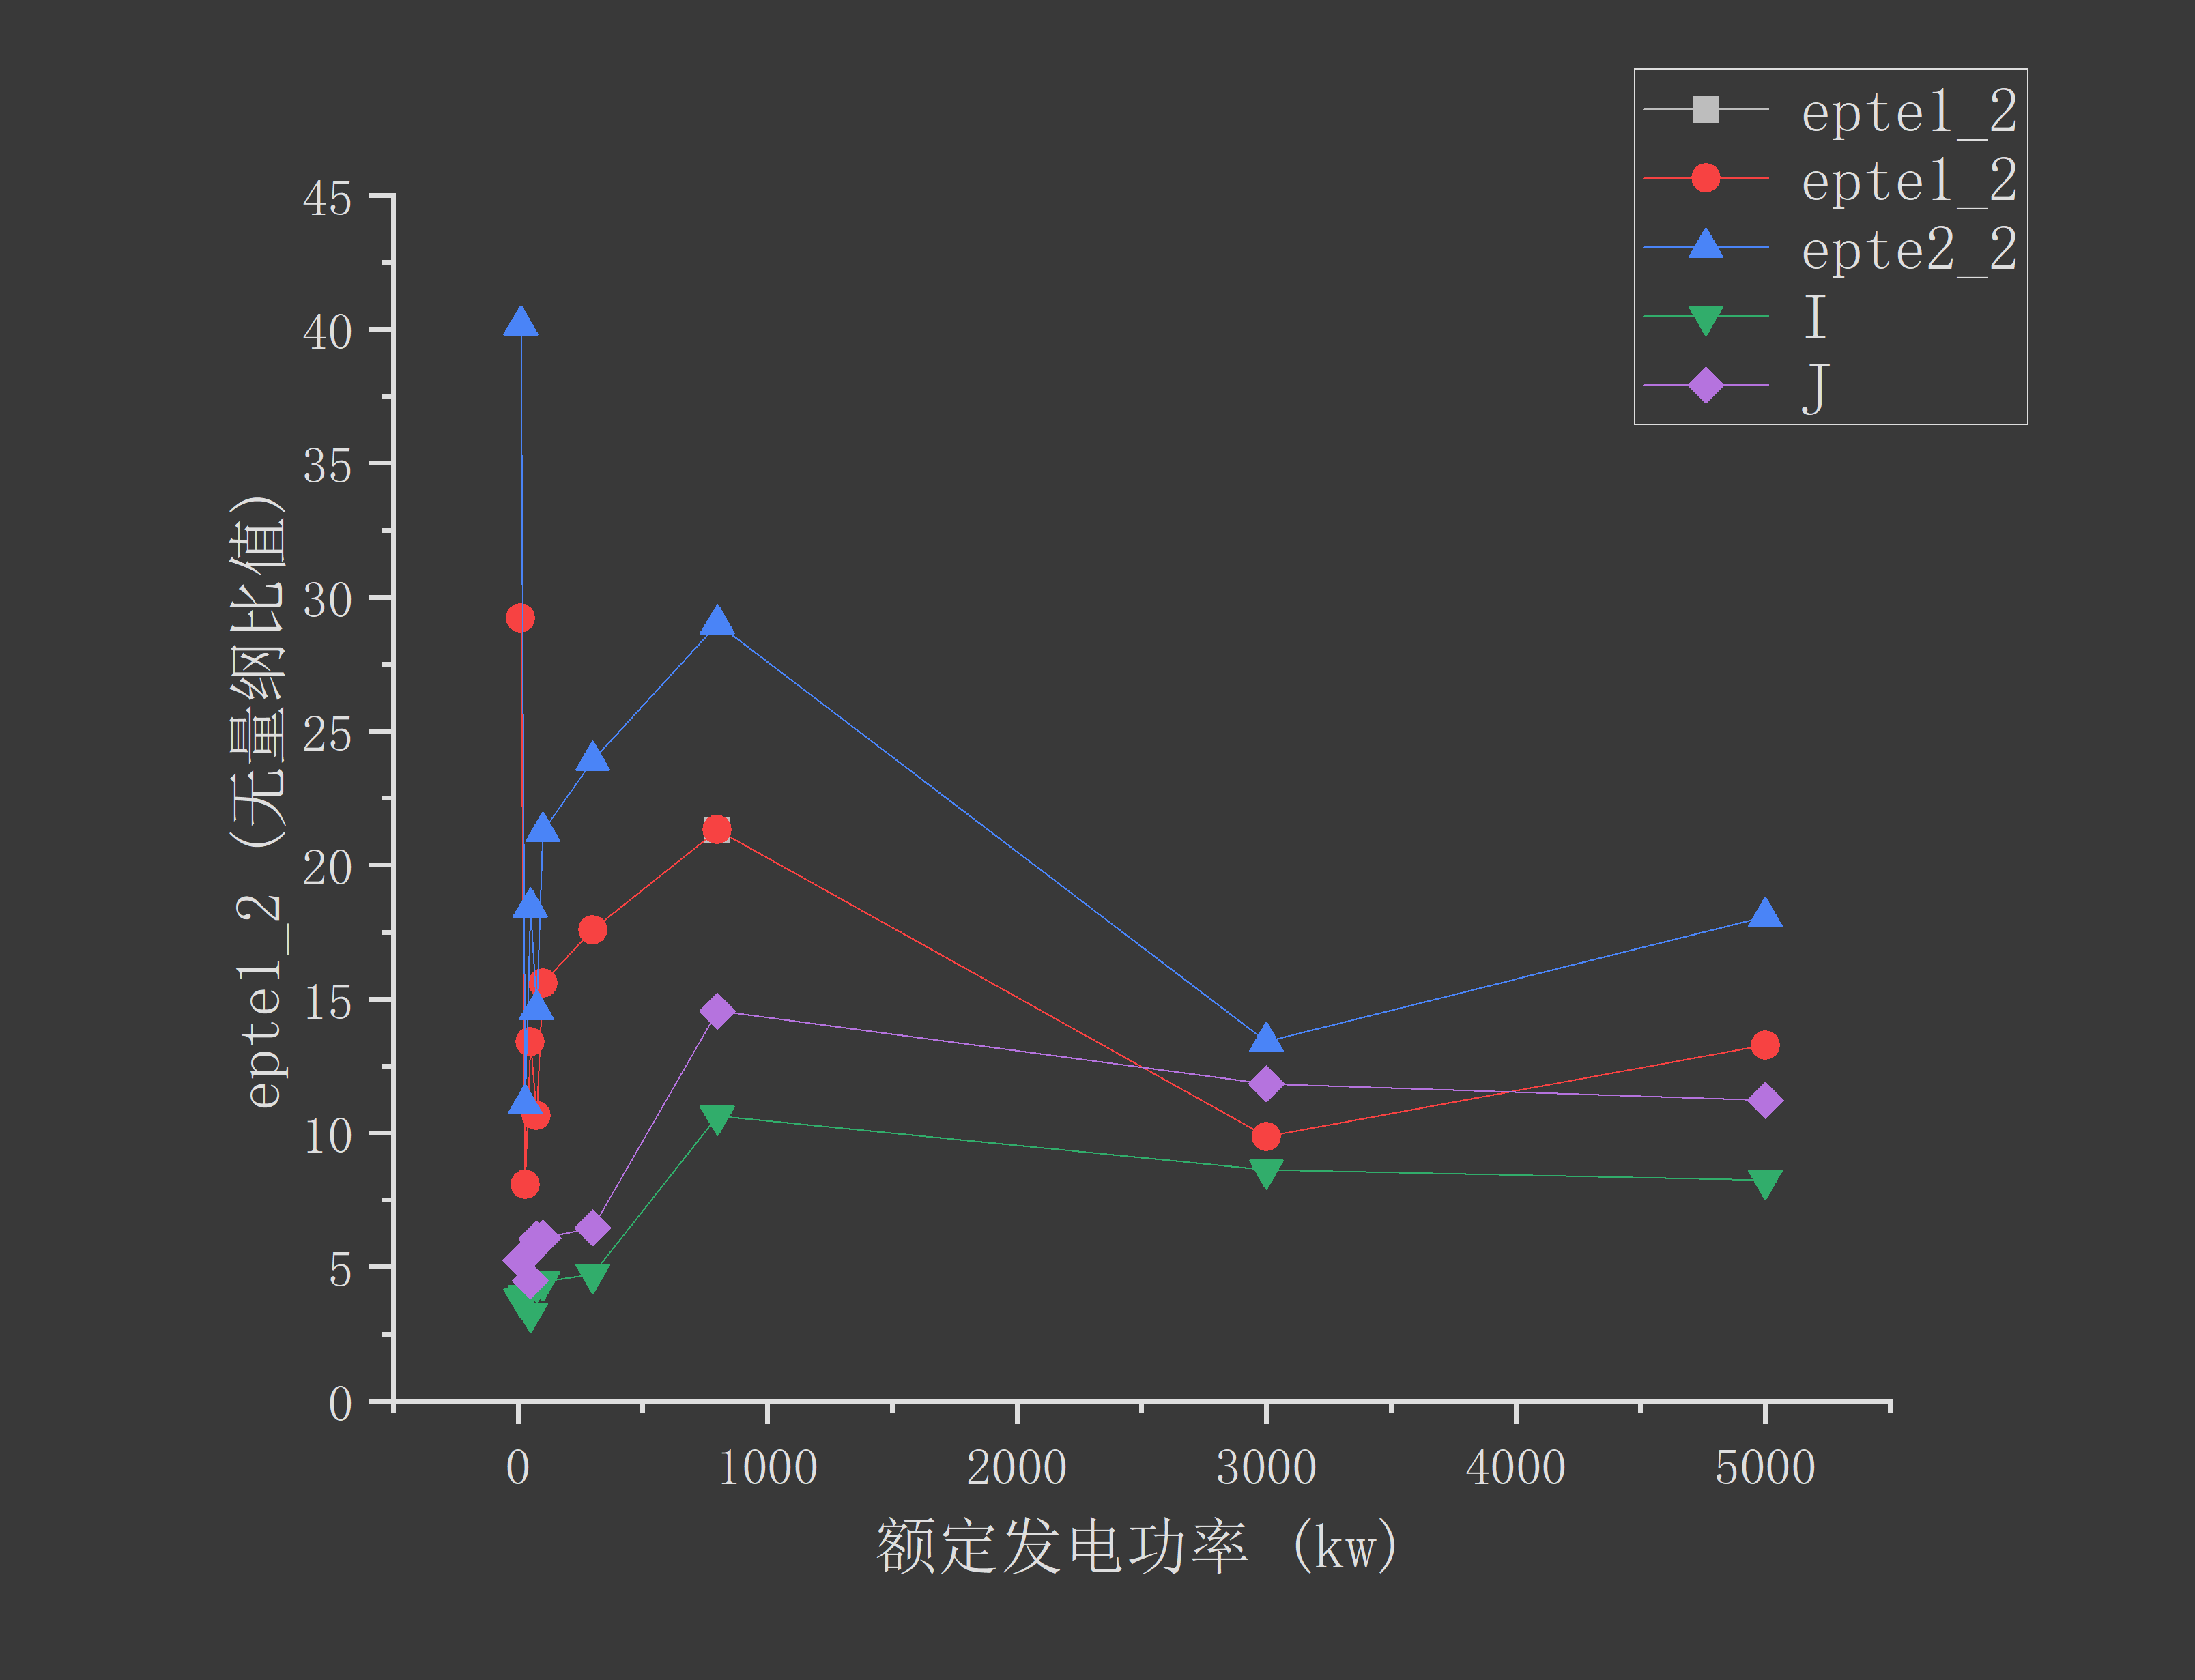
\includegraphics[width=0.9\textwidth]{fig/内燃机和汽轮机epte对比.png} % 替换为实际图片
  
  \caption{不同电价下燃气轮机与内燃机EPTE对比 (天然气价格2.5元/m³)}
  \label{fig:epte_elec_price}
\end{figure}

\textbf{分析讨论(预期):}
\begin{itemize}
    \item 通常情况下,EPTE值随功率增大有先增后降或持续增加的趋势,具体取决于初投资和运行效率的规模效应。
    \item 电价升高会显著提高系统的发电收益,从而整体提升EPTE值。
    \item 对比两种机组:在低功率段,可能内燃机因其相对较低的初投资和较高的部分负荷效率而表现出更好的经济性。在高功率段,燃气轮机的规模效应可能更显著。
    \item 需要观察是否存在一个交叉点,在该点前后两种机组的经济性发生反转。电价的变化可能会影响这个交叉点的位置。
\end{itemize}




\section{结论}
通过本次基于EPTE指标对燃气轮机和燃气内燃机冷热电联供系统的经济性比较分析,可以得到以下主要结论:
\textit{(根据上述分析结果,总结以下几点)}
\begin{enumerate}
    \item 两种机组(燃气轮机和燃气内燃机)的EPTE随额定功率变化的总体趋势如何?是否存在最优经济运行功率区间?
    \item 电价对两种机组EPTE的影响程度如何?高电价对哪种机组更有利?
    \item 天然气价格对两种机组EPTE的影响程度如何?高气价对哪种机组的经济性削弱更大?
    \item 在设定的不同能源价格情景和功率范围内,燃气轮机和燃气内燃机的经济性优劣对比如何?是否存在明显的适用性交叉点?
    \item 本研究对实际CCHP项目选型有何指导意义?
\end{enumerate}
例如:研究表明,在较低功率范围内(如P < XXX kW),燃气内燃机由于其XX特性,在YY能源价格条件下具有较高的EPTE值。而在较大功率范围(如P > XXX kW)或ZZ能源价格条件下,燃气轮机则显示出更好的经济性。电价的提升普遍有利于提高两种机组的经济性,但对XX机组的影响更为显著。天然气价格的上涨则对XX机组的EPTE冲击较大。因此,在进行CCHP系统方案选择时,应充分考虑项目的装机容量需求以及当地的能源价格水平。

\section*{附 录}
本次课程设计的计算和数据分析主要借助 OriginPro 软件进行数据拟合和图表绘制。
主要的Origin操作步骤包括:
\begin{enumerate}
    \item 将原始数据(额定功率、发电效率、热电效率、维修费用率、机组价格)导入Origin工作表。
    \item 选取对应的数据列,使用“Analysis”菜单下的“Fitting”功能,选择“Polynomial Fit”进行多项式拟合。
    \item 根据拟合结果(系数、R²值)评估拟合优度,并生成拟合曲线图。
    \item 将通过拟合公式计算得到的EPTE数据导入Origin,绘制EPTE随额定功率变化的对比曲线图。
\end{enumerate}
本报告中涉及的拟合曲线图和EPTE对比图均由Origin生成。
\begin{comment}
% 示例程序代码 (可以删除或保留作为格式参考)
\begin{verbatim}
% 假设的EPTE计算伪代码或关键公式 (如果需要)
function calculate_EPTE(Power, Price_elec, Price_fuel)
  % 利用拟合函数获取效率、成本等参数
  eta_e = fit_eta_e(Power);
  eta_th = fit_eta_th(Power);
  cost_maint_rate = fit_maint_rate(Power);
  invest_cost = fit_invest_cost(Power);
  
  % ... 执行章节2.2中的计算 ...
  
  Net_Income = Total_Revenue - Total_Expenditure;
  EPTE = Net_Income / invest_cost;
  return EPTE;
end
\end{verbatim}
\end{comment}

\newpage
% 成绩评定表
\section*{课程论文成绩评定表}
院系:化学工程与能源技术学院 \quad 班级:2023级能源与动力工程一班(化能杨班) \quad 姓名:唐玮嘉 \quad 学号:2023428020130 % 班级信息根据封面调整

\begin{tabularx}{\textwidth}{|l|X|c|p{2.2cm}|p{2.2cm}|p{2.2cm}|p{2.2cm}|p{2.2cm}|c|} % 调整列宽以适应页面
  \hline
  项目 & 子项目 & 分值 & 优秀($x \geq 90\%$) & 良好($90\% > x \geq 80\%$) & 中等($80\% > x \geq 70\%$) & 及格($70\% > x \geq 60\%$) & 不及格($x < 60\%$) & 评分 \\
  \hline
  平时考核 & 平时考核 & 20 & 学习态度认真,科学作风严谨,严格保证设计时间并按任务书中规定的进度开展各项工作。 & 学习态度比较认真,科学作风良好,能按期圆满完成任务书规定的任务。 & 学习态度尚好,遵守组织纪律,基本保证设计时间,按期完成各项工作。 & 学习态度尚可,能遵守组织纪律,能按期完成任务。 & 学习马虎,纪律涣散,工作作风不严谨,不能保证设计时间和进度。 & \\
  \hline
  \multirow{2}{*}{\begin{tabular}[c]{@{}l@{}}课程论文\\报告\end{tabular}} & 报告内容组织书写 & 40 & 结构严谨,逻辑性强,层次清晰,语言准确,文字流畅,完全符合规范化要求,书写工整或用计算机打印成文;图纸非常工整、清晰。 & 结构合理,符合逻辑,文章层次分明,语言准确,文字流畅,符合规范化要求,书写工整或用计算机打印成文;图纸工整、清晰。 & 结构合理,层次较为分明,文理通顺,基本达到规范化要求,书写比较工整;图纸比较工整、清晰。 & 结构基本合理,逻辑基本清楚,文字尚通顺,勉强达到规范化要求;图纸比较工整。 & 内容空泛,结构混乱,文字表达不清,错别字较多,达不到规范化要求;图纸不工整或不清晰。 & \\
  \cline{2-9}
  & 技术水平 & 40 & 设计合理、理论分析与计算正确,文献查阅能力强、引用合理、调查调研非常合理、可信。 & 设计合理、理论分析与计算正确,文献引用、调查调研比较合理、可信。 & 设计合理,理论分析与计算基本正确,主要文献引用、调查调研比较可信。 & 设计基本合理,理论分析与计算无大错。 & 设计不合理,理论分析与计算有原则错误,文献引用、调查调研有较大的问题。 & \\
  \hline
  \multicolumn{2}{|l|}{指导教师签名} & \multicolumn{7}{|l|}{\underline{\makebox[10cm][s]{}} 指导教师评定成绩:\underline{\makebox[3cm][s]{}}} \\ % 调整下划线长度
  \hline
\end{tabularx}

\end{document}